\chapter{Library Internals} \label{chap:internals}

Details about the internals of {\ViennaGrid} will be given in the following. 
They should aid developers to extend the library with additional features
and to understand the internal data structures used. 
Nevertheless, the information provided might be of interest for new users of {\ViennaGrid} as well.

\section{Recursive Inheritance}
{\ViennaGrid} extensively relies on recursive inheritance to build the individual element types.
The element are of type \lstinline|element_t<ElementTag, ConfigType>|, where \lstinline|ElementTag| is a tag identifying the topological shape of the element and \lstinline|ConfigType| is the configuration class. The class \lstinline|element_t| itself is almost empty, but
inherits the information about its boundary elements from a \lstinline|boundary_element_layer|. 
In addition, the class inherits from a class with the sole purpose of providing an ID mechanism
\begin{lstlisting}
 template <typename ElementTag,
           stypename ConfigType>
 class element_t :
    public viennagrid::storage::id_handler<...>,
    public boundary_element_layer<ElementTag, BoundaryElementContainerTypelist>,
 { ... }
\end{lstlisting}
The second template parameter of \lstinline|boundary_element_layer| is a typelist where all boundary element types are stored. The \lstinline|boundary_element_layer| inherits from a \lstinline|boundary_element_layer| with the last element type of that typelist.
\begin{lstlisting}
template<typename element_tag, typename bnd_cell_container_type_, typename orientation_container_type_, typename tail>
class boundary_element_layer<element_tag, meta::typelist_t< meta::static_pair<bnd_cell_container_type_, orientation_container_type_>, tail > > :
    public boundary_element_layer<element_tag, tail>
\end{lstlisting}
where the additional technical template arguments customizing the behavior of each boundary layer are omitted.
The recursion is terminated at vertex level by a partial template specialization of the class.

\begin{figure}[tb]
\centering
 \psfrag{element\_t}{\lstinline|element_t|}
 \psfrag{boundary\_element\_layer<facet tag>}{\lstinline|bnd_layer<facet>|}
 \psfrag{boundary\_element\_layer<facet of facet>}{\lstinline|bnd_layer<facet of facet>|}
 \psfrag{boundary\_element\_layer<vertex_tag>}{\lstinline|bnd_layer<vertex>|}
 \psfrag{ID}{\lstinline|ID|}
 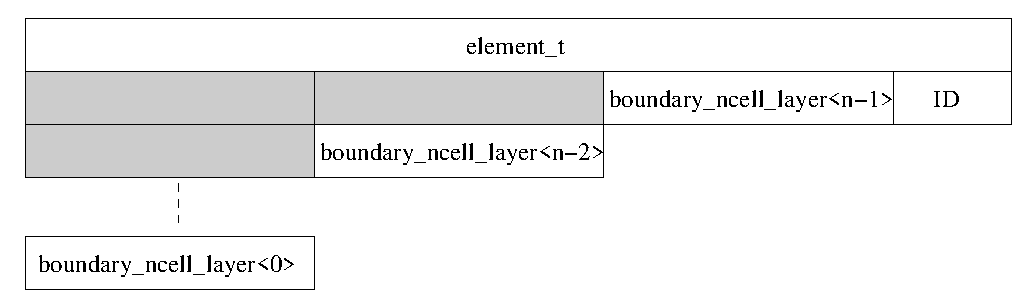
\includegraphics[width=0.95\textwidth]{figures/recursive-inheritance.eps}
 \caption{Illustration of recursive inheritance for the element class \lstinline|element_t|. The \lstinline|boundary_element_layer| class is abbreviated as \lstinline|bnd_layer|. The widths of the boxes refer to the sizes of a single class object.}
 \label{fig:recursive-inheritance}
\end{figure}
An illustration of the resulting class layout is given in Fig.~\ref{fig:recursive-inheritance}.
Since each layer is configured by respective metafunctions that return the specified user settings,
the class size of each layer varies depending on the storage of boundary cells and on the use of local reference orientations.

A problem of recursive inheritance is name hiding. For example, a member function \lstinline|fun()| defined for one layer
will be repeated in every layer and thus become inaccessible from the outside. The resolve this issue, member function overloading of the form
\begin{lstlisting}
 void fun(boundary_element_tag) { }
\end{lstlisting}
for boundary element with tag \lstinline|boundary_element_tag| is used. In this way, every layer is accessible from the outside, which is used for the free functions such as \lstinline|elements<>()|.

Domains and segments are set up in essentially the same way with a few internal storage facilities adjusted.
Instead of an ID handler, the segment inherits from a class providing a reference to the underlying domain.

\section{Element Storage in Domain and Segment}
For storing the elements inside a domain, the natural approach is to use a \lstinline|std::vector<>| for that purpose.
However, a drawback of this datastructure is that the number of elements should be known in advance in order to avoid
costly reallocations. This is especially a problem for mesh file formats which do not contain the total number of elements in an explicit way.
{\ViennaGrid} uses a \lstinline|std::deque<>| (double ended queue) as container for vertices and cells, because it does not suffer form costly reallocations
if the number of elements is a-priori unknown.

For non-vertices and non-cells, unique representations of the respective elements are required. For example, the edge connecting vertices $1$ and $2$ must not lead to an edge $[1,2]$ and an edge $[2,1]$ in the domain.
While such a distinction is simple for vertices, this is harder to achieve for e.g.~quadrilateral facets.
In {\ViennaGrid}, the global vertex IDs of each element are used as a tuple for the identification of the respective element.
Thus, the internal storage inside the domain for each non-vertices and non-cells is given by
\begin{lstlisting}
 std::map<TupleType, ElementType>
\end{lstlisting}
where \lstinline|TupleType| refers to the tuple of sorted global vertex IDs, and \lstinline|ElementType| is the type of the element.

For segments, only handles to the global element objects in the domain are stored.
Since uniqueness of elements is required in segments as well, an internal storage scheme of type \lstinline|std::set<ElementHandleType>| is chosen
for non-cells, where \lstinline|ElementType| denotes the type of the elements.

Finally, it should be noted that future versions of {\ViennaGrid} may provide additional flexibility in customizing the internal storage scheme for domain and segments.
In particular, users may be interested in replacing the \lstinline|std::map<TupleType, ElementType>| used for non-vertices and non-cells with a \lstinline|std::vector<>| after the setup phase for reasons of memory consumption, faster (random) access and/or better caching possibilities.



